\chapter{Implementación}

La implementación del software se ha dividido en hitos. Estos han sido definidos en GitHub
y cada uno de ellos contiene un grupo de \textit{issues} que se corresponden con las distintas
mejoras que se han ido incorporando al software a lo largo de su desarrollo.

\section{Hito 0. Infraestructura y planificación}

Se realizó la planificación inicial que se puede encontrar redactada en el capítulo \ref{ch:planning} y organizada en el \href{https://github.com/dipzza/ultrastar-song2txt}{repositorio} del proyecto. Además, se configuraron las siguientes herramientas.


\subsection{Integración Continua}

Se consideraron varios servicios que permiten \textbf{automatizar los procesos de integración continua} en la nube, con la condición de que dispongan de planes gratuitos para proyectos de código abierto y buscando el servicio más sencillo de integrar con el repositorio del proyecto en GitHub.

Tanto Travis CI,  Circle CI y GitHub Actions ofrecen planes gratuitos. Se considera que GitHub Actions es el servicio que mejor cumple las características deseadas, debido a su integración dentro de la propia interfaz de GitHub, la facilidad de configuración y la posibilidad de reusar flujos de trabajo públicos (también llamados acciones). Los otros servicios poseen ventajas, como soporte para otras plataformas en las que alojar el código o diferencias en los precios de los planes de pago, pero para este proyecto se consideran irrelevantes.

Utilizando el servicio escogido se han configurado una serie de flujos de trabajo que son ejecutados cada vez que se introducen cambios en cualquier rama de desarrollo.

\subsubsection{Memoria}

\paragraph*{Compilación de archivos de LaTeX.}

La memoria del trabajo ha sido escrita con LaTeX, un sistema de composición de textos comúnmente usado en artículos académicos, tesis y libros técnicos por su calidad tipográfica y amplias capacidades.

Es necesario compilar los archivos de LaTeX para obtener el documento final. Por ello, se ha configurado un flujo de trabajo para \textbf{comprobar que la compilación se completa sin errores}. El flujo realiza un paso adicional si la rama principal de desarrollo está afectada (ya sea por introducir cambios o por hacerse un \textit{pull request} a esta) que \textbf{almacena el documento final generado}.

\paragraph*{Corrección de la memoria.}

Para asegurar una correcta redacción de la memoria se ha utilizado la herramienta de software libre \href{https://github.com/sylvainhalle/textidote}{TeXtidote}. A diferencia de otras herramientas que solo revisan la ortografía (Aspell, Ispell...) se puede configurar para que \textbf{revise la ortografía, la gramática e incluso el estilo} tanto en la redacción como en la propia sintaxis de LaTeX.

Con la intención de hacer las \textbf{comprobaciones más extensas y estrictas}, se ha definido un flujo de trabajo con todos los tests posibles de TeXtidote tanto para el \textbf{texto en Inglés como para el texto en Español}, introduciendo excepciones para algunas palabras y reglas para ignorar construcciones de LaTeX. Además de indicar el número de errores encontrados, el flujo \textbf{almacena un informe detallado} de los resultados en formato HTML.


\subsubsection{Código}

\paragraph*{Análisis estático.}

Configurar un \textit{linter} (herramienta que lleva a cabo un análisis estático del código para detectar errores) es un paso básico para garantizar la calidad del código.

Se busca un \textit{linter} fácil de configurar, que detecte errores de programación y compruebe la adherencia a la guía de estilo \href{https://peps.python.org/pep-0008/}{PEP8}.

Existen multitud de opciones que proveen estas funcionalidades, o parte de ellas, para código escrito en Python (pycodestyle, pylint, pyflakes, flake8,...). Se ha escogido flake8 porque además de agrupar la funcionalidad deseada al detectar errores de programación y estilísticos, incluye comprobaciones sobre la complejidad del código y es rápida.

\paragraph*{Test unitarios y de integración.}
\label{sec:tests}

Es necesario un marco de pruebas para escribir y automatizar la ejecución de test unitarios (testean que cada parte de la aplicación funcione como se espera de forma aislada) y test de integración (testean que distintas partes de la aplicación trabajando juntas funcionan como se espera).

Se han considerado pytest y unittest como marcos de pruebas, ambas opciones satisfacen las características requeridas.

Finalmente, se ha elegido pytest debido a que posee una sintaxis más simple, lo que ayuda a la comprensión de los test que se definan, y, a diferencia de unittest, el nombre de sus funciones respeta la guía de estilo PEP8. Además, cuenta con un complemento para revisar la cobertura del código que proporcionan los test.

\paragraph*{Flujo configurado.}

Se ha definido un flujo de trabajo que verifica que el proyecto y sus dependencias se instalan correctamente, que las comprobaciones del \textit{linter} no reportan ningún error y que los test escritos se ejecutan sin errores cubriendo un porcentaje significativo del código (al menos el 85\%).

\subsection{Gestión de dependencias y empaquetado}
\label{sec:poetry}

Un \textbf{entorno de desarrollo reproducible} que defina sus dependencias
(librerías de códigos o paquetes que son reusados en un proyecto) es fundamental para asegurarnos de que los programas funcionan igual independientemente del equipo en el que se ejecuten.

Para ello se busca una herramienta para la gestión de \textbf{entornos virtuales} (entornos aislados que no dependen del resto del sistema), \textbf{dependencias}, el \textbf{empaquetado} y \textbf{publicación}.

Además de proporcionar esta funcionalidad se espera que la herramienta sea simple, rápida y use el formato de archivo de configuración TOML, establecido como estándar en las propuestas de mejora de Python \href{https://peps.python.org/pep-0517/}{PEP517}, \href{https://peps.python.org/pep-0518/}{PEP518} y \href{https://peps.python.org/pep-0621/}{PEP621}.

Existen multitud de opciones (pip, venv, pipenv, setuptools, distutils, Poetry...), pipenv posee las características esperadas, pero solo para la gestión de entornos virtuales y dependencias, la única que agrupa toda la funcionalidad necesaria y utiliza un único fichero TOML para toda la configuración es \textbf{Poetry} y, por lo tanto, esta es la herramienta que se ha utilizado.

La principal desventaja de Poetry es que no está tan extendida, suponiendo para un usuario que esté acostumbrado a otras herramientas tener que instalar y aprender una nueva. Para paliar este inconveniente \textbf{se provee en el repositorio el archivo \texttt{requirements.txt}} que especifica las mismas dependencias que el archivo \texttt{poetry.lock} de Poetry en un formato apto \textbf{para poder instalar las dependencias con otras herramientas}.


\subsection{Gestor de tareas}

Los gestores de tareas son herramientas útiles para construir software de calidad porque permiten \textbf{automatizar y hacer reproducibles las tareas del desarrollo}.  

La cualidad principal que se desea en un gestor de tareas para este proyecto es \textbf{versatilidad}, es decir, que permita \textbf{lanzar órdenes en el intérprete de comandos} directamente.  Esto nos permitiría definir tareas no solo para la construcción de la aplicación, sino también para una variedad de procesos que se llevan a cabo en el desarrollo y que dependen de otros programas.

Hay una gran variedad de gestores de tareas que satisfacen este requisito y, por lo tanto, serían opciones viables (make, Task, taskipy, mmake, poethepoet...).

No es necesaria la funcionalidad extra que proveen algunas de las herramientas, por ello, buscando la comodidad de los desarrolladores, \textbf{se ha escogido la herramienta más conocida}, instalada por defecto en la mayoría de distribuciones de Linux,  \textbf{make}.

Se ha creado un \textit{Makefile} (archivo de texto donde se definen las tareas ejecutables)  en la carpeta del proyecto con la \textbf{definición de tareas} para la realización de test, la instalación, el empaquetado y la distribución \textbf{del código}, y otro archivo en la carpeta de la documentación para la compilación y la realización de test sobre los archivos \textbf{de LaTeX}.


\subsection{Contribuyendo de vuelta a proyectos libres}

Una de las muchas \textbf{ventajas del software libre} es que puedes \textbf{contribuir a solucionar los problemas} que encuentres tu mismo. Durante el desarrollo de este hito se hicieron algunas contribuciones pequeñas.

\begin{enumerate}
	\item{Inicialmente, los informes sobre la corrección de la memoria contenían falsos positivos, debido a una \textbf{dependencia desactualizada} en la acción de GitHub usada. Se presentó un \textit{pull request} arreglando el problema que fue integrado el mismo día por el mantenedor del repositorio original. \href{https://github.com/ChiefGokhlayeh/textidote-action/pull/33}{Enlace al \textit{pull request}}.}
	
	\item{Se encontró un error en TeXtidote en el que el programa no tenía el comportamiento esperado e \textbf{ignoraba un comando de LaTeX}. Tras hacer un reporte del error el desarrollador principal proporciono indicaciones sobre una posible solución. Con la información proporcionada, se implementó una solución con soporte para las distintas sintaxis del comando y, tras testear el correcto funcionamiento del programa, se presentó un \textit{pull request}. \href{https://github.com/sylvainhalle/textidote/issues/208}{Enlace al \textit{issue}}. \href{https://github.com/sylvainhalle/textidote/pull/209}{Enlace al \textit{pull request}}.}
	
	\item{Para poder revisar los idiomas empleados en la memoria con TeXtidote fue necesario aplicar una solución algo enrevesada. Con la intención de mejorar este caso de uso se propuso una implementación para el \textbf{soporte de múltiples lenguajes} en un \textit{issue}, que \textbf{ha sido añadido como parte del siguiente hito del proyecto}. \href{https://github.com/sylvainhalle/textidote/issues/203}{Enlace al \textit{issue}}.}
	
	\item{Finalmente, se hizo un \textit{pull request} para \textbf{corregir un error de sintaxis} en la \textbf{plantilla de LaTeX} empleada. \href{https://github.com/JJ/plantilla-TFG-ETSIIT/pull/7}{Enlace al \textit{pull request}}.}
\end{enumerate}

\section{Hito 1. Estimación de tonos}

\subsection{Estructura del proyecto}
Para organizar los archivos de la aplicación se deseaba una estructura simple, fácil para trabajar con ella y de entender.  La estructura "plana" o "\textit{adhoc}"  ejemplificada en la figura \ref{fig:layout1} usa una cantidad reducida de carpetas y profundidad que aun así organiza los archivos de forma lógica.  Por ello, se han organizado los archivos según esta estructura  que cumple los requisitos y es reconocida sin configuración adicional por herramientas usadas en el proyecto como Poetry (sección \ref{sec:poetry}) o Pytest (sección \ref{sec:tests}).

\begin{figure}[h]
	\centering
	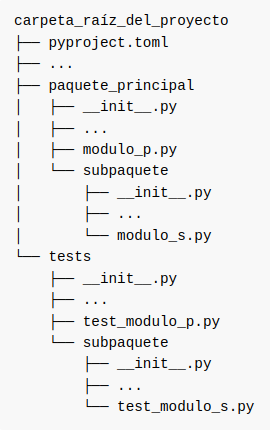
\includegraphics[width=0.5\linewidth]{logos/layout.png}
	\caption{Ejemplo de estructura plana}
	\label{fig:layout1}
\end{figure}


\subsection{Librería para trabajar con archivos UltraStar txt}

Para poder empezar a construir la aplicación es necesario poder trabajar con los archivos de texto que definen las canciones de karaoke. Concretamente, con el formato de texto estándar UltraStar txt \footnote{https://github.com/UltraStar-Deluxe/Play/wiki/UltraStar-txt-File-Format},  utilizado por la mayoría de videojuegos de karaoke libres, incluidos los mencionados en la sección \ref{sec:motivation}.

Con esta intención, se ha construido una librería para leer este tipo de archivos transformando el texto a estructuras de datos apropiadas para trabajar con ellas y para escribir nuevos archivos generando el texto correspondiente a partir de las estructuras de datos.

\subsubsection{Lectura del archivo}

En la definición del formato UltraStar txt no se establece la codificación de caracteres que deben usar los archivos, y como resultado, se comparten con distintas codificaciones. Tampoco es posible determinar la codificación a partir del archivo de forma sencilla, ya que son archivos de texto plano donde no se encuentra especificada.

Buscando la mayor compatibilidad se consideraron los siguientes acercamientos para decodificar los archivos:

\begin{itemize}
	\item{Probar a decodificar el texto por cada codificación posible hasta que todos los caracteres se descodifiquen sin ningún error.}
	\item{Utilizar una librería que estime la codificación más probable para el contenido del archivo.}
	\begin{itemize}
		\item{Chardet}
		\item{cChardet}
		\item{Charset Normalizer}
	\end{itemize}
\end{itemize}

Inicialmente, se consideró usar la primera opción porque no añadía dependencias al proyecto. Sin embargo, era posible que se acabara utilizando una codificación que no generara ningún error, pero interpretara incorrectamente algunos caracteres (por ejemplo el carácter \texttt{"ñ"} podía ser interpretado incorrectamente como \texttt{"ń"}).

Por este motivo se decidió usar el segundo acercamiento y así obtener una fiabilidad mayor. Teniendo en cuenta las pruebas de rendimiento disponibles en la \href{https://github.com/Ousret/charset_normalizer}{web} de Charset Normalizer y el tamaño de cada librería la opción más adecuada a las necesidades del proyecto es Charset Normalizer, ya que, presenta la mayor precisión y el menor tamaño de las opciones consideradas.

La implementación final estima el formato de codificación del archivo de texto entre varias opciones comunes (el formato estándar UTF-8 definido en la \href{https://www.rfc-editor.org/rfc/rfc3629}{RFC 3629} y aquellos usados por defecto en versiones antiguas del sistema operativo Windows). Si aun así no se decodificara el texto correctamente, como última opción, el usuario podría utilizar la utilidad de la línea de comandos incluida con Charset Normalizer para transformar el archivo de texto a UTF-8 seleccionando manualmente la interpretación correcta.

\subsubsection{Estructuras de datos}

Como plantillas para las estructuras de datos se han definido las clases representadas en la figura \ref{fig:class1}, intentando crear capas de abstracción adecuadas al dominio del problema. Además, se han definido algunos comportamientos asociados:
\begin{itemize}
	\item{Comprobaciones de que los valores que se asignen son válidos (por ejemplo, la duración de una nota no puede ser negativa) tanto en creación como en modificación, en caso contrario, se indica el problema lanzando una excepción del tipo correspondiente con un mensaje que explica el error.}
	\item{Métodos para generar el texto que correspondería en un archivo UltraStar txt a partir de los datos almacenados en el objeto.}
	\item{Implementación del método \texttt{\_\_eq\_\_} para poder comparar objetos  y determinar si son iguales.}
\end{itemize}

\begin{figure}[H]
	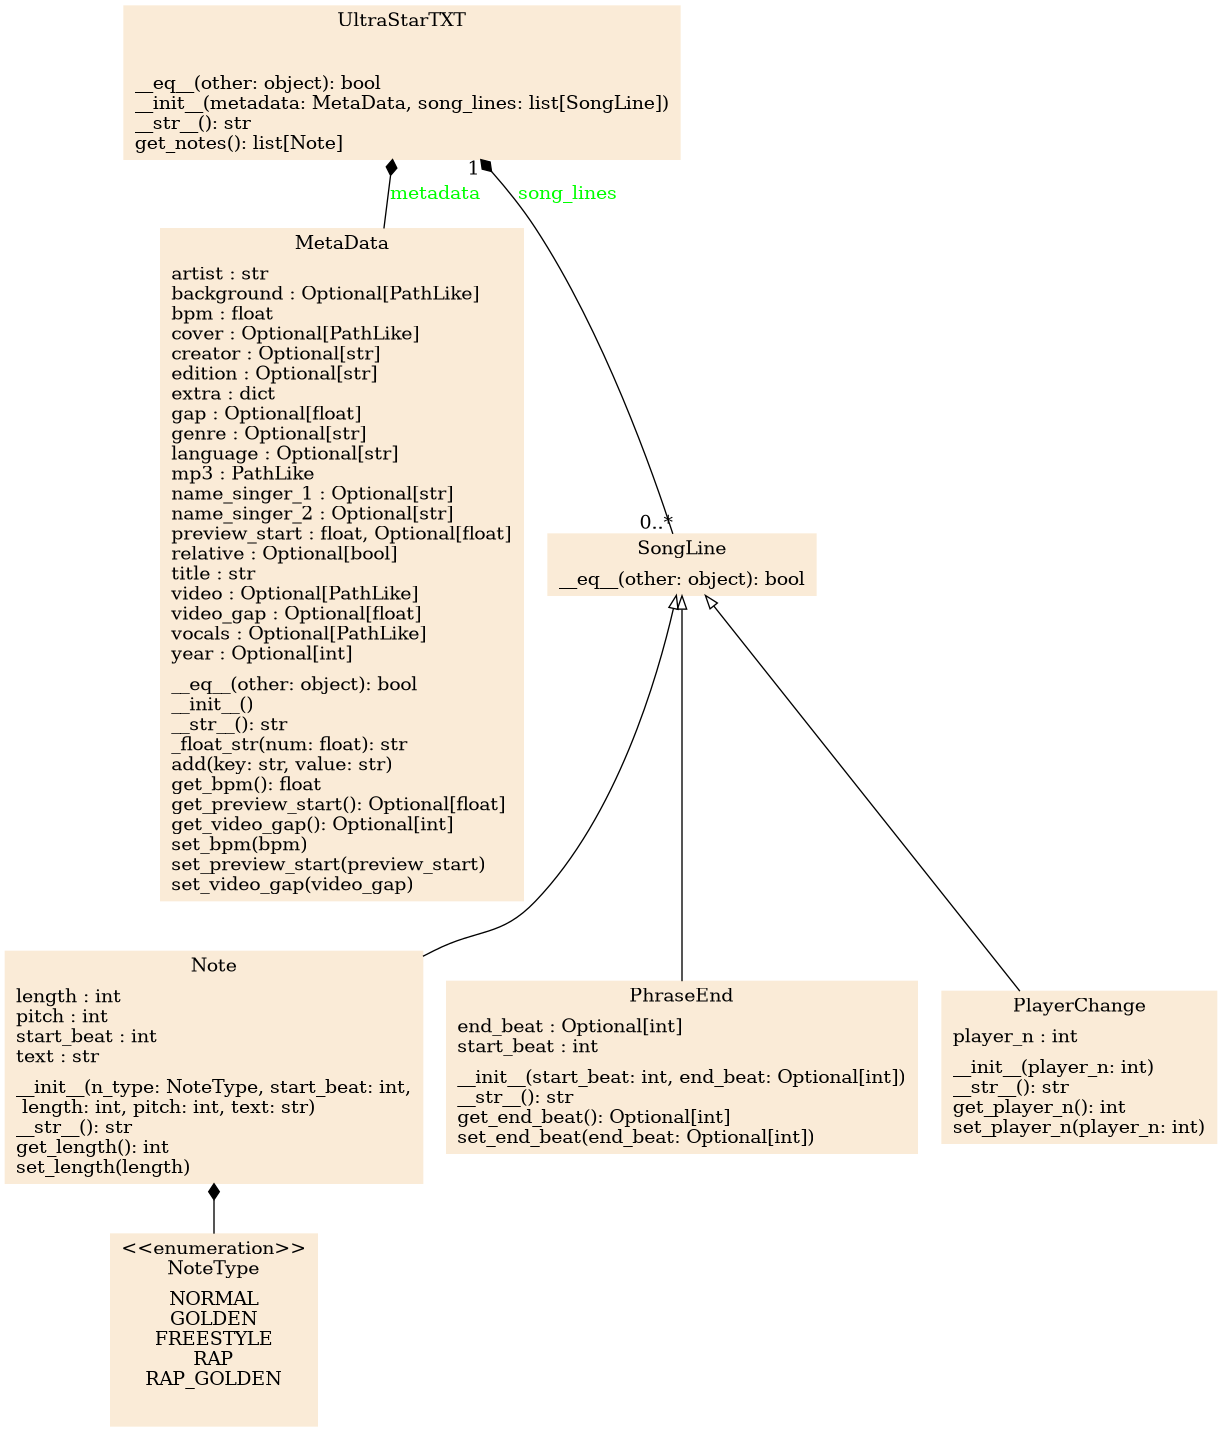
\includegraphics[width=\linewidth]{logos/classes.png}
	\caption{Diagrama de clases}
	\label{fig:class1}
\end{figure}

\subsubsection{Extracción de datos del texto}

Se desea separar y extraer los fragmentos de texto que contienen la información relevante, para poder convertirlos a las estructuras de datos definidas. Buscando un método fácil de mantener y que permita garantizar que el texto de entrada presenta un formato correcto se han considerado las siguientes opciones:

\begin{itemize}
	\item{Operaciones básicas de transformación de texto, como separar por cada espacio, para quedarnos con una lista de los valores que necesitamos.}
	\item{Expresiones regulares para definir y detectar patrones.}
	\item{Módulos externos para generar un analizador del texto a partir de una definición de la gramática.}
\end{itemize}


Para escoger la opción más adecuada es importante tener en cuenta que el formato del texto presenta un lenguaje regular, sencillo y sin anidado. Para este tipo de lenguaje las expresiones regulares son adecuadas permitiendo validar fácilmente que el texto presenta el formato correcto (a diferencia de las transformaciones básicas de texto) y siendo una solución corta, simple y precisa (a diferencia de los módulos de analizadores de propósito general, que son más adecuados para gramáticas complejas).

Por lo tanto, la implementación realizada procesa cada línea por orden utilizando expresiones regulares (ya que cada fragmento de información se encuentra separado en una línea distinta) y transforma la información extraída en objetos de las clases definidas anteriormente, componiendo finalmente un solo objeto que contiene toda la información del archivo de texto.  Si el formato del texto es incorrecto, ya sea por no respetar el orden (primero un bloque de metadatos, después descripción de la canción) o porque alguna línea no coincide con ninguna de las expresiones regulares, se lanza una excepción indicando el error y mostrando el número de línea que lo ha causado y su contenido.

